% !TEX root = ../../ctfp-print.tex

\lettrine[lhang=0.17]{T}{he category of types and functions} plays an important role in
programming, so let's talk about what types are and why we need them.

\section{Who Needs Types?}

There seems to be some controversy about the advantages of static vs.
dynamic and strong vs. weak typing. Let me illustrate these choices with
a thought experiment. Imagine millions of monkeys at computer keyboards
happily hitting random keys, producing programs, compiling, and running
them.

\begin{figure}[H]
  \centering
  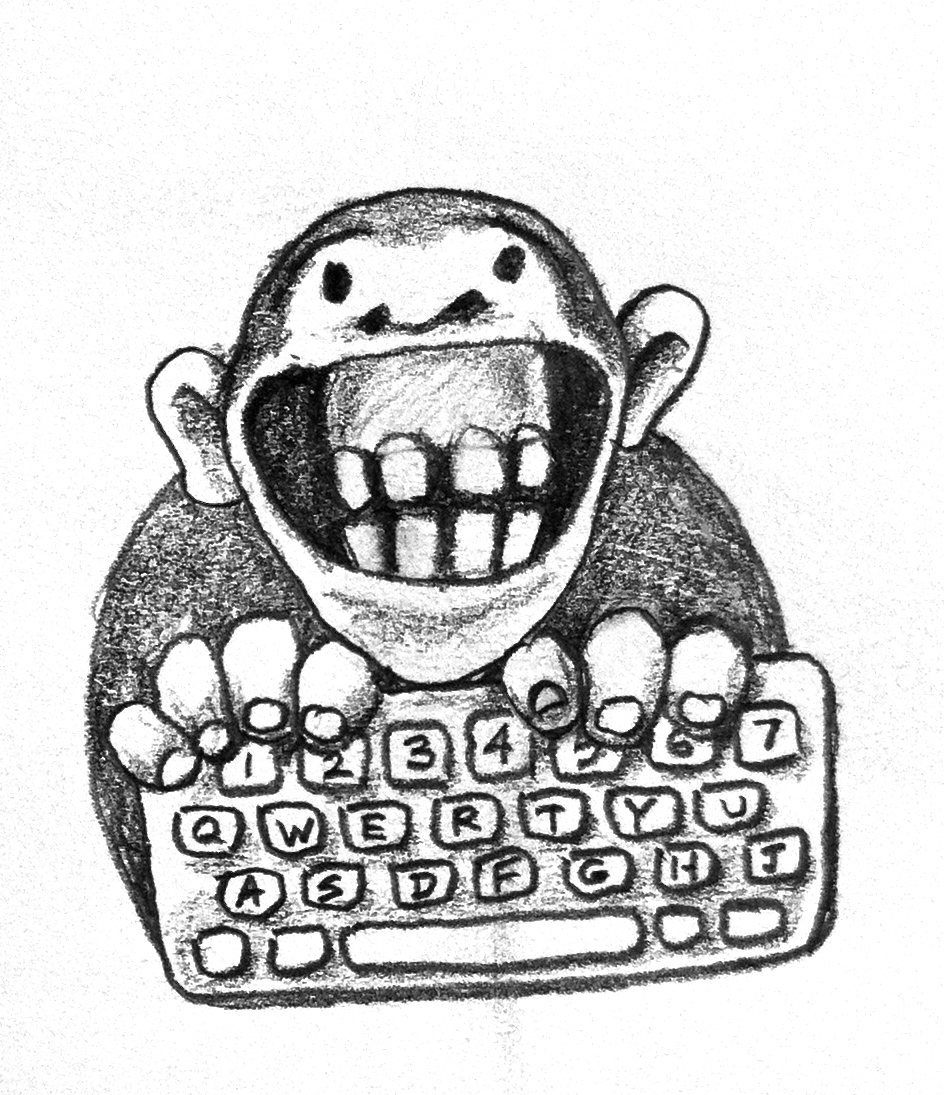
\includegraphics[width=0.3\textwidth]{images/img_1329.jpg}
\end{figure}

\noindent
With machine language, any combination of bytes produced by monkeys
would be accepted and run. But with higher level languages, we do
appreciate the fact that a compiler is able to detect lexical and
grammatical errors. Lots of monkeys will go without bananas, but the
remaining programs will have a better chance of being useful. Type
checking provides yet another barrier against nonsensical programs.
Moreover, whereas in a dynamically typed language, type mismatches would
be discovered at runtime, in strongly typed statically checked languages,
type mismatches are discovered at compile time, eliminating lots of
incorrect programs before they have a chance to run.

So the question is, do we want to make monkeys happy, or do we want to
produce correct programs?

The usual goal in the typing monkeys thought experiment is the
production of the complete works of Shakespeare. Having a spell checker
and a grammar checker in the loop would drastically increase the odds.
The analog of a type checker would go even further by making sure that,
once Romeo is declared a human being, he doesn't sprout leaves or trap
photons in his powerful gravitational field.

\section{Types Are About Composability}

Category theory is about composing arrows. But not any two arrows can be
composed. The target object of one arrow must be the same as the source
object of the next arrow. In programming we pass the results of
one function to another. The program will not work if the target
function is not able to correctly interpret the data produced by the
source function. The two ends must fit for the composition to work. The
stronger the type system of the language, the better this match can be
described and mechanically verified.

The only serious argument I hear against strong static type checking is
that it might eliminate some programs that are semantically correct. In
practice, this happens extremely rarely and, in any case, every language
provides some kind of a backdoor to bypass the type system when that's
really necessary. Even Haskell has \code{unsafeCoerce}. But such
devices should be used judiciously. Franz Kafka's character, Gregor
Samsa, breaks the type system when he metamorphoses into a giant bug,
and we all know how it ends.

Another argument I hear a lot is that dealing with types imposes too
much burden on the programmer. I could sympathize with this sentiment
after having to write a few declarations of iterators in C++ myself,
except that there is a technology called \newterm{type inference} that lets
the compiler deduce most of the types from the context in which they are
used. In C++, you can now declare a variable \code{auto} and let the
compiler figure out its type.

In Haskell, except on rare occasions, type annotations are purely
optional. Programmers tend to use them anyway, because they can tell a
lot about the semantics of code, and they make compilation errors easier
to understand. It's a common practice in Haskell to start a project by
designing the types. \sloppy{Later, type annotations drive the implementation
  and become compiler-enforced comments.}

Strong static typing is often used as an excuse for not testing the
code. You may sometimes hear Haskell programmers saying, ``If it
compiles, it must be correct.'' Of course, there is no guarantee that a
type-correct program is correct in the sense of producing the right
output. The result of this cavalier attitude is that in several studies
Haskell didn't come as strongly ahead of the pack in code quality as one
would expect. It seems that, in the commercial setting, the pressure to
fix bugs is applied only up to a certain quality level, which has
everything to do with the economics of software development and the
tolerance of the end user, and very little to do with the programming
language or methodology. A better criterion would be to measure how many
projects fall behind schedule or are delivered with drastically reduced
functionality.

As for the argument that unit testing can replace strong typing,
consider the common refactoring practice in strongly typed languages:
changing the type of an argument of a particular function. In a strongly
typed language, it's enough to modify the declaration of that function
and then fix all the build breaks. In a weakly typed language, the fact
that a function now expects different data cannot be propagated to call
sites. Unit testing may catch some of the mismatches, but testing is
almost always a probabilistic rather than a deterministic process.
Testing is a poor substitute for proof.

\section{What Are Types?}

The simplest intuition for types is that they are sets of values. The
type \code{Bool} (remember, concrete types start with a capital letter
in Haskell) is a two-element set of \code{True} and \code{False}.
Type \code{Char} is a set of all Unicode characters like
\code{a} or \code{ą}.

Sets can be finite or infinite. The type of \code{String}, which is a
synonym for a list of \code{Char}, is an example of an infinite set.

When we declare \code{x} to be an \code{Integer}:

\src{snippet01}
we are saying that it's an element of the set of integers.
\code{Integer} in Haskell is an infinite set, and it can be used to do
arbitrary precision arithmetic. There is also a finite-set \code{Int}
that corresponds to machine type, just like the C++ \code{int}.

There are some subtleties that make this identification of types and
sets tricky. There are problems with polymorphic functions that involve
circular definitions, and with the fact that you can't have a set of all
sets; but as I promised, I won't be a stickler for math. The great thing
is that there is a category of sets, which is called $\Set$, and
we'll just work with it. In $\Set$, objects are sets and morphisms
(arrows) are functions.

$\Set$ is a very special category, because we can actually peek
inside its objects and get a lot of intuitions from doing that. For
instance, we know that an empty set has no elements. We know that there
are special one-element sets. We know that functions map elements of one
set to elements of another set. They can map two elements to one, but
not one element to two. We know that an identity function maps each
element of a set to itself, and so on. The plan is to gradually forget
all this information and instead express all those notions in purely
categorical terms, that is in terms of objects and arrows.

In the ideal world we would just say that Haskell types are sets and
Haskell functions are mathematical functions between sets. There is just
one little problem: A mathematical function does not execute any code
--- it just knows the answer. A Haskell function has to calculate the
answer. It's not a problem if the answer can be obtained in a finite
number of steps --- however big that number might be. But there are some
calculations that involve recursion, and those might never terminate. We
can't just ban non-terminating functions from Haskell because
distinguishing between terminating and non-terminating functions is
undecidable --- the famous halting problem. That's why computer
scientists came up with a brilliant idea, or a major hack, depending on
your point of view, to extend every type by one more special value
called the \newterm{bottom} and denoted by \code{\_|\_}, or
Unicode $\bot$. This ``value'' corresponds to a non-terminating computation.
So a function declared as:

\src{snippet02}
may return \code{True}, \code{False}, or \code{\_|\_};
the latter meaning that it would never terminate.

Interestingly, once you accept the bottom as part of the type system, it
is convenient to treat every runtime error as a bottom, and even allow
functions to return the bottom explicitly. The latter is usually done
using the expression \code{undefined}, as in:

\src{snippet03}
This definition type checks because \code{undefined} evaluates to
bottom, which is a member of any type, including \code{Bool}. You can
even write:

\src{snippet04}
(without the \code{x}) because the bottom is also a member of the type
\code{Bool -> Bool}.

Functions that may return bottom are called partial, as opposed to total
functions, which return valid results for every possible argument.

Because of the bottom, you'll see the category of Haskell types and
functions referred to as $\Hask$ rather than $\Set$. From
the theoretical point of view, this is the source of never-ending
complications, so at this point I will use my butcher's knife and
terminate this line of reasoning. From the pragmatic point of view, it's
okay to ignore non-terminating functions and bottoms, and treat
$\Hask$ as bona fide $\Set$.\footnote{Nils Anders Danielsson,
  John Hughes, Patrik Jansson, Jeremy Gibbons, \href{http://www.cs.ox.ac.uk/jeremy.gibbons/publications/fast+loose.pdf}{
    Fast and Loose Reasoning is Morally Correct}. This paper provides justification for ignoring bottoms in most contexts.}

\section{Why Do We Need a Mathematical Model?}

As a programmer you are intimately familiar with the syntax and grammar
of your programming language. These aspects of the language are usually
described using formal notation at the very beginning of the language
spec. But the meaning, or semantics, of the language is much harder to
describe; it takes many more pages, is rarely formal enough, and almost
never complete. Hence the never ending discussions among language
lawyers, and a whole cottage industry of books dedicated to the exegesis
of the finer points of language standards.

There are formal tools for describing the semantics of a language but,
because of their complexity, they are mostly used with simplified
academic languages, not real-life programming behemoths. One such tool
called \newterm{operational semantics} describes the mechanics of program
execution. It defines a formalized idealized interpreter. The semantics
of industrial languages, such as C++, is usually described using
informal operational reasoning, often in terms of an ``abstract
machine.''

The problem is that it's very hard to prove things about programs using
operational semantics. To show a property of a program you essentially
have to ``run it'' through the idealized interpreter.

It doesn't matter that programmers never perform formal proofs of
correctness. We always ``think'' that we write correct programs. Nobody
sits at the keyboard saying, ``Oh, I'll just throw a few lines of code
and see what happens.'' We think that the code we write will perform
certain actions that will produce desired results. We are usually quite
surprised when it doesn't. That means we do reason about programs we
write, and we usually do it by running an interpreter in our heads. It's
just really hard to keep track of all the variables. Computers are good
at running programs --- humans are not! If we were, we wouldn't need
computers.

But there is an alternative. It's called \newterm{denotational semantics}
and it's based on math. In denotational semantics every programming
construct is given its mathematical interpretation. With that, if you
want to prove a property of a program, you just prove a mathematical
theorem. You might think that theorem proving is hard, but the fact is
that we humans have been building up mathematical methods for thousands
of years, so there is a wealth of accumulated knowledge to tap into.
Also, as compared to the kind of theorems that professional
mathematicians prove, the problems that we encounter in programming are
usually quite simple, if not trivial.

Consider the definition of a factorial function in Haskell, which is a
language quite amenable to denotational semantics:

\src{snippet05}
The expression \code{{[}1..n{]}} is a list of integers from \code{1} to \code{n}.
The function \code{product} multiplies all elements of a list. That's
just like a definition of factorial taken from a math text. Compare this
with C:

\begin{snip}{c}
int fact(int n) {
    int i;
    int result = 1;
    for (i = 2; i <= n; ++i)
        result *= i;
    return result;
}
\end{snip}
Need I say more?

Okay, I'll be the first to admit that this was a cheap shot! A factorial
function has an obvious mathematical denotation. An astute reader might
ask: What's the mathematical model for reading a character from the
keyboard or sending a packet across the network? For the longest time
that would have been an awkward question leading to a rather convoluted
explanation. It seemed like denotational semantics wasn't the best fit
for a considerable number of important tasks that were essential for
writing useful programs, and which could be easily tackled by
operational semantics. The breakthrough came from category theory.
Eugenio Moggi discovered that computational effect can be mapped to
monads. This turned out to be an important observation that not only
gave denotational semantics a new lease on life and made pure functional
programs more usable, but also shed new light on traditional
programming. I'll talk about monads later, when we develop more
categorical tools.

One of the important advantages of having a mathematical model for
programming is that it's possible to perform formal proofs of
correctness of software. This might not seem so important when you're
writing consumer software, but there are areas of programming where the
price of failure may be exorbitant, or where human life is at stake. But
even when writing web applications for the health system, you may
appreciate the thought that functions and algorithms from the Haskell
standard library come with proofs of correctness.

\section{Pure and Dirty Functions}

The things we call functions in C++ or any other imperative language,
are not the same things mathematicians call functions. A mathematical
function is just a mapping of values to values.

We can implement a mathematical function in a programming language: Such
a function, given an input value will calculate the output value. A
function to produce a square of a number will probably multiply the
input value by itself. It will do it every time it's called, and it's
guaranteed to produce the same output every time it's called with the
same input. The square of a number doesn't change with the phases of the
Moon.

Also, calculating the square of a number should not have a side effect
of dispensing a tasty treat for your dog. A ``function'' that does that
cannot be easily modelled as a mathematical function.

In programming languages, functions that always produce the same result
given the same input and have no side effects are called \newterm{pure
  functions}. In a pure functional language like Haskell all functions are
pure. Because of that, it's easier to give these languages denotational
semantics and model them using category theory. As for other languages,
it's always possible to restrict yourself to a pure subset, or reason
about side effects separately. Later we'll see how monads let us model
all kinds of effects using only pure functions. So we really don't lose
anything by restricting ourselves to mathematical functions.

\section{Examples of Types}

Once you realize that types are sets, you can think of some rather
exotic types. For instance, what's the type corresponding to an empty
set? No, it's not C++ \code{void}, although this type \emph{is} called
\code{Void} in Haskell. It's a type that's not inhabited by any
values. You can define a function that takes \code{Void}, but you can
never call it. To call it, you would have to provide a value of the type
\code{Void}, and there just aren't any. As for what this function can
return, there are no restrictions whatsoever. It can return any type
(although it never will, because it can't be called). In other words
it's a function that's polymorphic in the return type. Haskellers have a
name for it:

\src{snippet06}
(Remember, \code{a} is a type variable that can stand for any type.)
The name is not coincidental. There is deeper interpretation of types
and functions in terms of logic called the Curry-Howard isomorphism. The
type \code{Void} represents falsity, and the type of the function
\code{absurd} corresponds to the statement that from falsity follows
anything, as in the Latin adage ``ex falso sequitur quodlibet.''

Next is the type that corresponds to a singleton set. It's a type that
has only one possible value. This value just ``is.'' You might not
immediately recognize it as such, but that is the C++ \code{void}.
Think of functions from and to this type. A function from \code{void}
can always be called. If it's a pure function, it will always return the
same result. Here's an example of such a function:

\begin{snip}{c}
int f44() { return 44; }
\end{snip}
You might think of this function as taking ``nothing'', but as we've
just seen, a function that takes ``nothing'' can never be called because
there is no value representing ``nothing.'' So what does this function
take? Conceptually, it takes a dummy value of which there is only one
instance ever, so we don't have to mention it explicitly. In Haskell,
however, there is a symbol for this value: an empty pair of parentheses,
\code{()}. So, by a funny coincidence (or is it a coincidence?), the
call to a function of void looks the same in C++ and in Haskell. Also,
because of the Haskell's love of terseness, the same symbol \code{()}
is used for the type, the constructor, and the only value corresponding
to a singleton set. So here's this function in Haskell:

\src{snippet07}
The first line declares that \code{f44} takes the type \code{()},
pronounced ``unit,'' into the type \code{Integer}. The second line
defines \code{f44} by pattern matching the only constructor for unit,
namely \code{()}, and producing the number 44. You call this function
by providing the unit value \code{()}:

\begin{snip}{c}
f44 ()
\end{snip}
Notice that every function of unit is equivalent to picking a single
element from the target type (here, picking the \code{Integer} 44). In
fact you could think of \code{f44} as a different representation for
the number 44. This is an example of how we can replace explicit mention
of elements of a set by talking about functions (arrows) instead.
Functions from unit to any type $A$ are in one-to-one correspondence with
the elements of that set $A$.

What about functions with the \code{void} return type, or, in Haskell,
with the unit return type? In C++ such functions are used for side
effects, but we know that these are not real functions in the
mathematical sense of the word. A pure function that returns unit does
nothing: it discards its argument.

Mathematically, a function from a set $A$ to a singleton set maps every
element of $A$ to the single element of that singleton set. For every $A$
there is exactly one such function. Here's this function for
\code{Integer}:

\src{snippet08}
You give it any integer, and it gives you back a unit. In the spirit of
terseness, Haskell lets you use the wildcard pattern, the underscore,
for an argument that is discarded. This way you don't have to invent a
name for it. So the above can be rewritten as:

\src{snippet09}
Notice that the implementation of this function not only doesn't depend
on the value passed to it, but it doesn't even depend on the type of the
argument.

Functions that can be implemented with the same formula for any type are
called parametrically polymorphic. You can implement a whole family of
such functions with one equation using a type parameter instead of a
concrete type. What should we call a polymorphic function from any type
to unit type? Of course we'll call it \code{unit}:

\src{snippet10}
In C++ you would write this function as:

\begin{snip}{cpp}
template<typename T>
void unit(T) {}
\end{snip}
Next in the typology of types is a two-element set. In C++ it's called
\code{bool} and in Haskell, predictably, \code{Bool}. The difference
is that in C++ \code{bool} is a built-in type, whereas in Haskell it
can be defined as follows:

\src{snippet11}
(The way to read this definition is that \code{Bool} is either
\code{True} or \code{False}.) In principle, one should also be able
to define a Boolean type in C++ as an enumeration:

\begin{snip}{cpp}
enum bool {
    true,
    false
};
\end{snip}
but C++ \code{enum} is secretly an integer. The C++11
``\code{enum class}'' could have been used instead, but then you
would have to qualify its values with the class name, as in
\code{bool::true} and \code{bool::false}, not to mention having to
include the appropriate header in every file that uses it.

Pure functions from \code{Bool} just pick two values from the target
type, one corresponding to \code{True} and another to \code{False}.

Functions to \code{Bool} are called \newterm{predicates}. For instance,
the Haskell library \code{Data.Char} is full of predicates like
\code{isAlpha} or \code{isDigit}. In C++ there is a similar library
\code{} that defines, among others, \code{isalpha} and
\code{isdigit}, but these return an \code{int} rather than a
Boolean. The actual predicates are defined in \code{std::ctype} and
have the form \code{ctype::is(alpha, c)}, \code{ctype::is(digit, c)}, etc.

\section{Challenges}

\begin{enumerate}
  \tightlist
  \item
        Define a higher-order function (or a function object) \code{memoize}
        in your favorite language. This function takes a pure function
        \code{f} as an argument and returns a function that behaves almost
        exactly like \code{f}, except that it only calls the original
        function once for every argument, stores the result internally, and
        subsequently returns this stored result every time it's called with
        the same argument. You can tell the memoized function from the
        original by watching its performance. For instance, try to memoize a
        function that takes a long time to evaluate. You'll have to wait for
        the result the first time you call it, but on subsequent calls, with
        the same argument, you should get the result immediately.
  \item
        Try to memoize a function from your standard library that you normally
        use to produce random numbers. Does it work?
  \item
        Most random number generators can be initialized with a seed.
        Implement a function that takes a seed, calls the random number
        generator with that seed, and returns the result. Memoize that
        function. Does it work?
  \item
        Which of these C++ functions are pure? Try to memoize them and observe
        what happens when you call them multiple times: memoized and not.

        \begin{enumerate}
          \tightlist
          \item
                The factorial function from the example in the text.
          \item
                \begin{minted}{cpp}
std::getchar()
\end{minted}
          \item
                \begin{minted}{cpp}
bool f() {
    std::cout << "Hello!" << std::endl;
    return true;
}
\end{minted}
          \item
                \begin{minted}{cpp}
int f(int x) {
    static int y = 0;
    y += x;
    return y;
}
\end{minted}
        \end{enumerate}
  \item
        How many different functions are there from \code{Bool} to
        \code{Bool}? Can you implement them all?
  \item
        Draw a picture of a category whose only objects are the types
        \code{Void}, \code{()} (unit), and \code{Bool}; with arrows
        corresponding to all possible functions between these types. Label the
        arrows with the names of the functions.
\end{enumerate}
